%!TEX root = ./Latihan/main.tex

\documentclass{article}
\usepackage[indonesian]{babel}
\usepackage{lipsum}
\usepackage{nccmath}
\usepackage{tikz, pgfplots}
\pgfplotsset{compat=1.18} 
\usepackage{amsmath,amssymb}
\usepackage{graphicx}
\usepackage{standalone}

% config untuk apa
\usepackage{apacite}
\usepackage[backend=biber, style=apa]{biblatex}
\addbibresource{eg.bib}


\begin{document}

\section{Hasil dan pembahasan (refresh dari hasil.tex}
    \label{sec:hasil}
    \begin{figure}[htbp]
      \centering
      \begin{tikzpicture}
        \draw (-1,0)--(1,0);
        \draw[dashed] (0,0)--(0,-2);
        \draw (0,0)--(-65:2) node[midway,right] {$L$};
        \fill (-65:2) circle (0.1);
      \end{tikzpicture}\label{pic:ayunan}
      \caption{Pengukuran panjang ayunan}\label{fig:alat}
    \end{figure}

    \begin{figure}[htb]
        \centering
        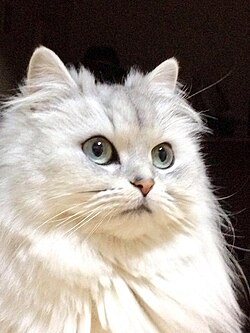
\includegraphics[width=0.2\linewidth]{Latihan/gambar/Persian_silver_dollface.jpg}
        \caption{Caption}
        \label{fig:placeholder}
    \end{figure}
    Satu periode adalah $T=t/N$, dengan $N$ jumlah getaran.
    \begin{equation}\label{eq:periode}
    T \approx 2\pi\sqrt{\frac{L}{g}}.
    \end{equation}

    \begin{fleqn}
        \begin{align}
        \int f(x) \, dx = F(x) + C
        \end{align}
    \end{fleqn}

    % \begin{freqn}
    %     \begin{align}
    %         \frac{dF(x)}{dx} = f(x)
    %     \end{align}
    % \end{freqn}
            
    Persamaan~\ref{eq:periode} dan persamaan~\eqref{eq:periode} pada subbab \ref{sec:hasil} berlaku untuk sudut kecil.

\end{document}